\section{Diagrama de Estados}

\par O diagrama de estado representa os possíveis estados, sendo alterado pelas operações que são executados dentro do sistema I-Library.

\subsection{\labeltext[Diagrama de Estados - Levantamento]{Diagrama de estados - Levantamento}{es:250}}

\begin{figure}[H]
	\centering
	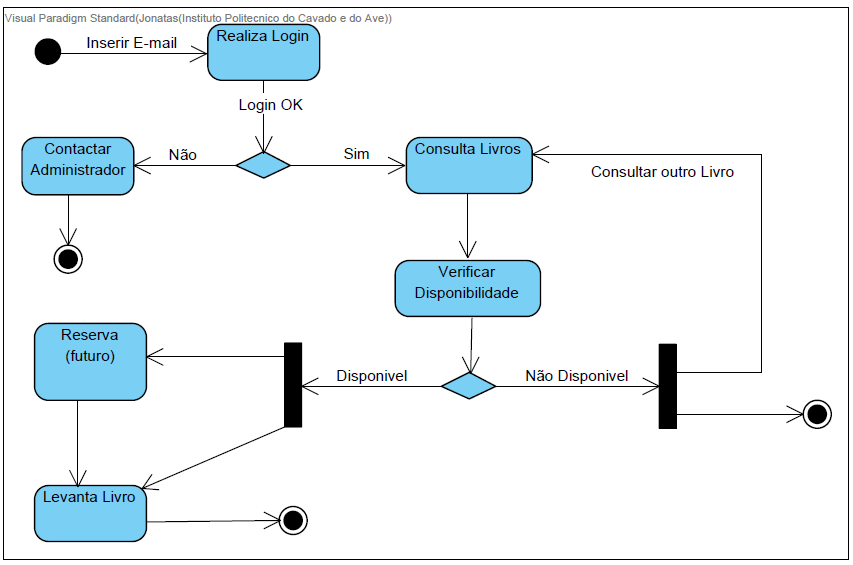
\includegraphics[width=1\linewidth]{./img/Diagrama_E/DE_Requisicao.png}  % largura percentual 
	\caption{\ref{es:250}}
	\label{fig:chap250}
\end{figure}

\par O diagrama de “Levantamento” inicia no estado "Realiza login", na falha de login o estado altera para “Contactar Administrador” e, após o processo finaliza, no caso de os dados estarem corretos o estado altera para “Consulta Livros”, após a ação do usuário o estado altera para “Verificar Disponibilidade”, deste momento, temos dois estados distintos, ou seja, caso tenha disponibilidade o estado altera para “Reserva Futuras” e após para “Levanta Livro”, neste sentido o estado finaliza, no caso de não haver disponibilidade o estado para altera para o fim.

%DE_Devolução
\subsection{\labeltext[Diagrama de Estados - Devolução]{Diagrama de estados - Devolução}{es:251}}

\begin{figure}[H]
	\centering
	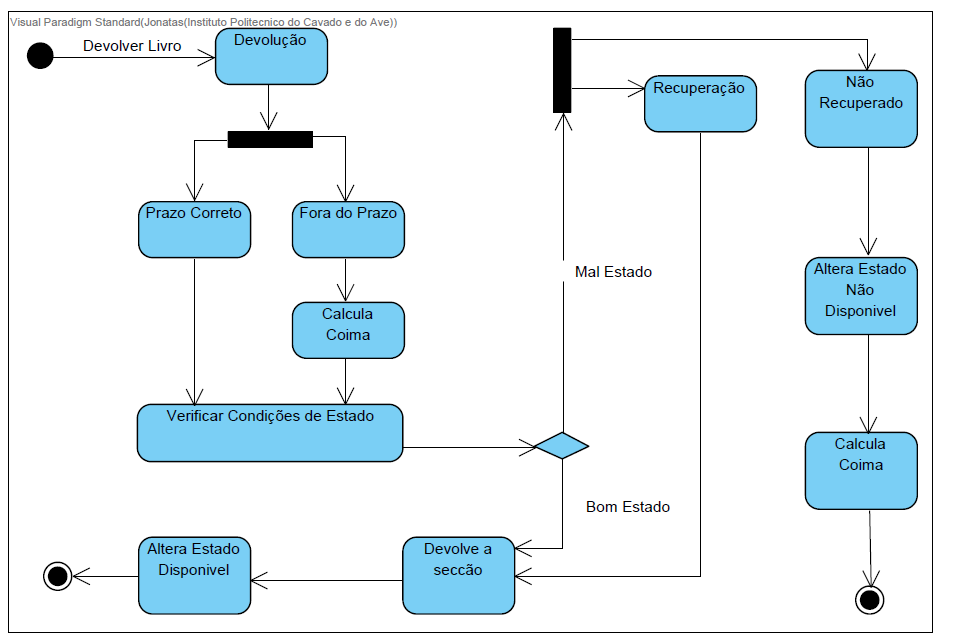
\includegraphics[width=1\linewidth]{./img/Diagrama_E/DE_Devolucao.png}  % largura percentual 
	\caption{\ref{es:251}}
	\label{fig:chap251}
\end{figure}

\par O diagrama de “Devolução” inicia no estado "Devolução", quando este está no “Prazo Correto” o estado segue para “Verificar condições de Estado”, na ocasião de estar “Fora do Prazo” o estado altera para “Calcula Coima”  e, segue para “Verificar condições de Estado”, quando este livro está em boas condições o estado altera para “Devolve a Secção” e após “Altera Estado para Disponível” e finaliza o processo, quando o livro encontra-se em mal condição o estado altera para “Recuperação” e caso seja possível o reparo volta para o estado de “Devolve a Secção”, já no caso de “Não Recuperado” o estado “Altera Estado para Não Disponível” e segue para “Calcula Coima” após o processo finaliza.

\newpage

%DE_Pagamento
\subsection{\labeltext[Diagrama de Estados - Pagamento]{Diagrama de estados - Pagamento}{es:252}}

\begin{figure}[H]
	\centering
	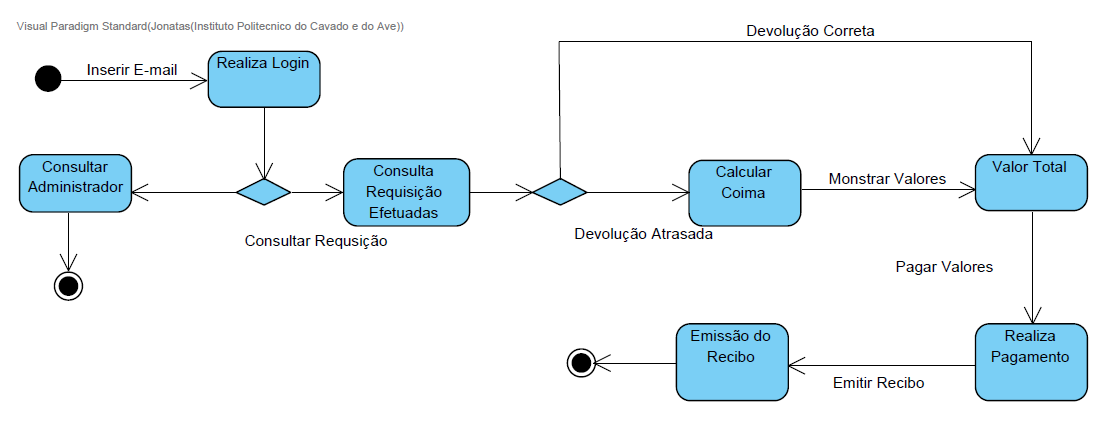
\includegraphics[width=1\linewidth]{./img/Diagrama_E/DE_Pagamento.png}  % largura percentual 
	\caption{\ref{es:252}}
	\label{fig:chap252}
\end{figure}

\par O diagrama de “Pagamento” inicia no estado de "Realiza login", na falha de login o estado altera para “Contactar Administrador” e, após o processo finaliza, no caso de login correto o estado altera “Consulta Requisição Efetuadas” neste momento o usuário terá acesso a todas suas requisições e, no caso de devolução atrasada o estado altera para “Calcular Coima” onde altera o estado para “Valor Total”, deste modo, o sistema altera o estado para “Realiza Pagamento”, após efetuado altera para “Emissão do Recibo”, sendo após finalizado o processo.

\newpage